\newpage
\section{Resultados, Mediciones y Verificación} \label{sec:4_resmedver}

% -----------------------------------------------------------------------------------------------%
\subsection{Parámetros de Dispersión Medidos}
Las Figuras~\ref{fig:s11_meas} y \ref{fig:s21_meas} presentan los parámetros $S_{11}$ y $S_{21}$ simulados y medidos, respectivamente, en el rango de DC a 5\,GHz. En la respuesta medida se identificó una resonancia fuera de la banda de interés. Esta característica no fue predicha por el modelo de simulación original y se atribuye a efectos parásitos del layout de la placa y del empaquetado de los componentes que no fueron completamente capturados en el modelo inicial.

\begin{figure}[H]
    \centering
    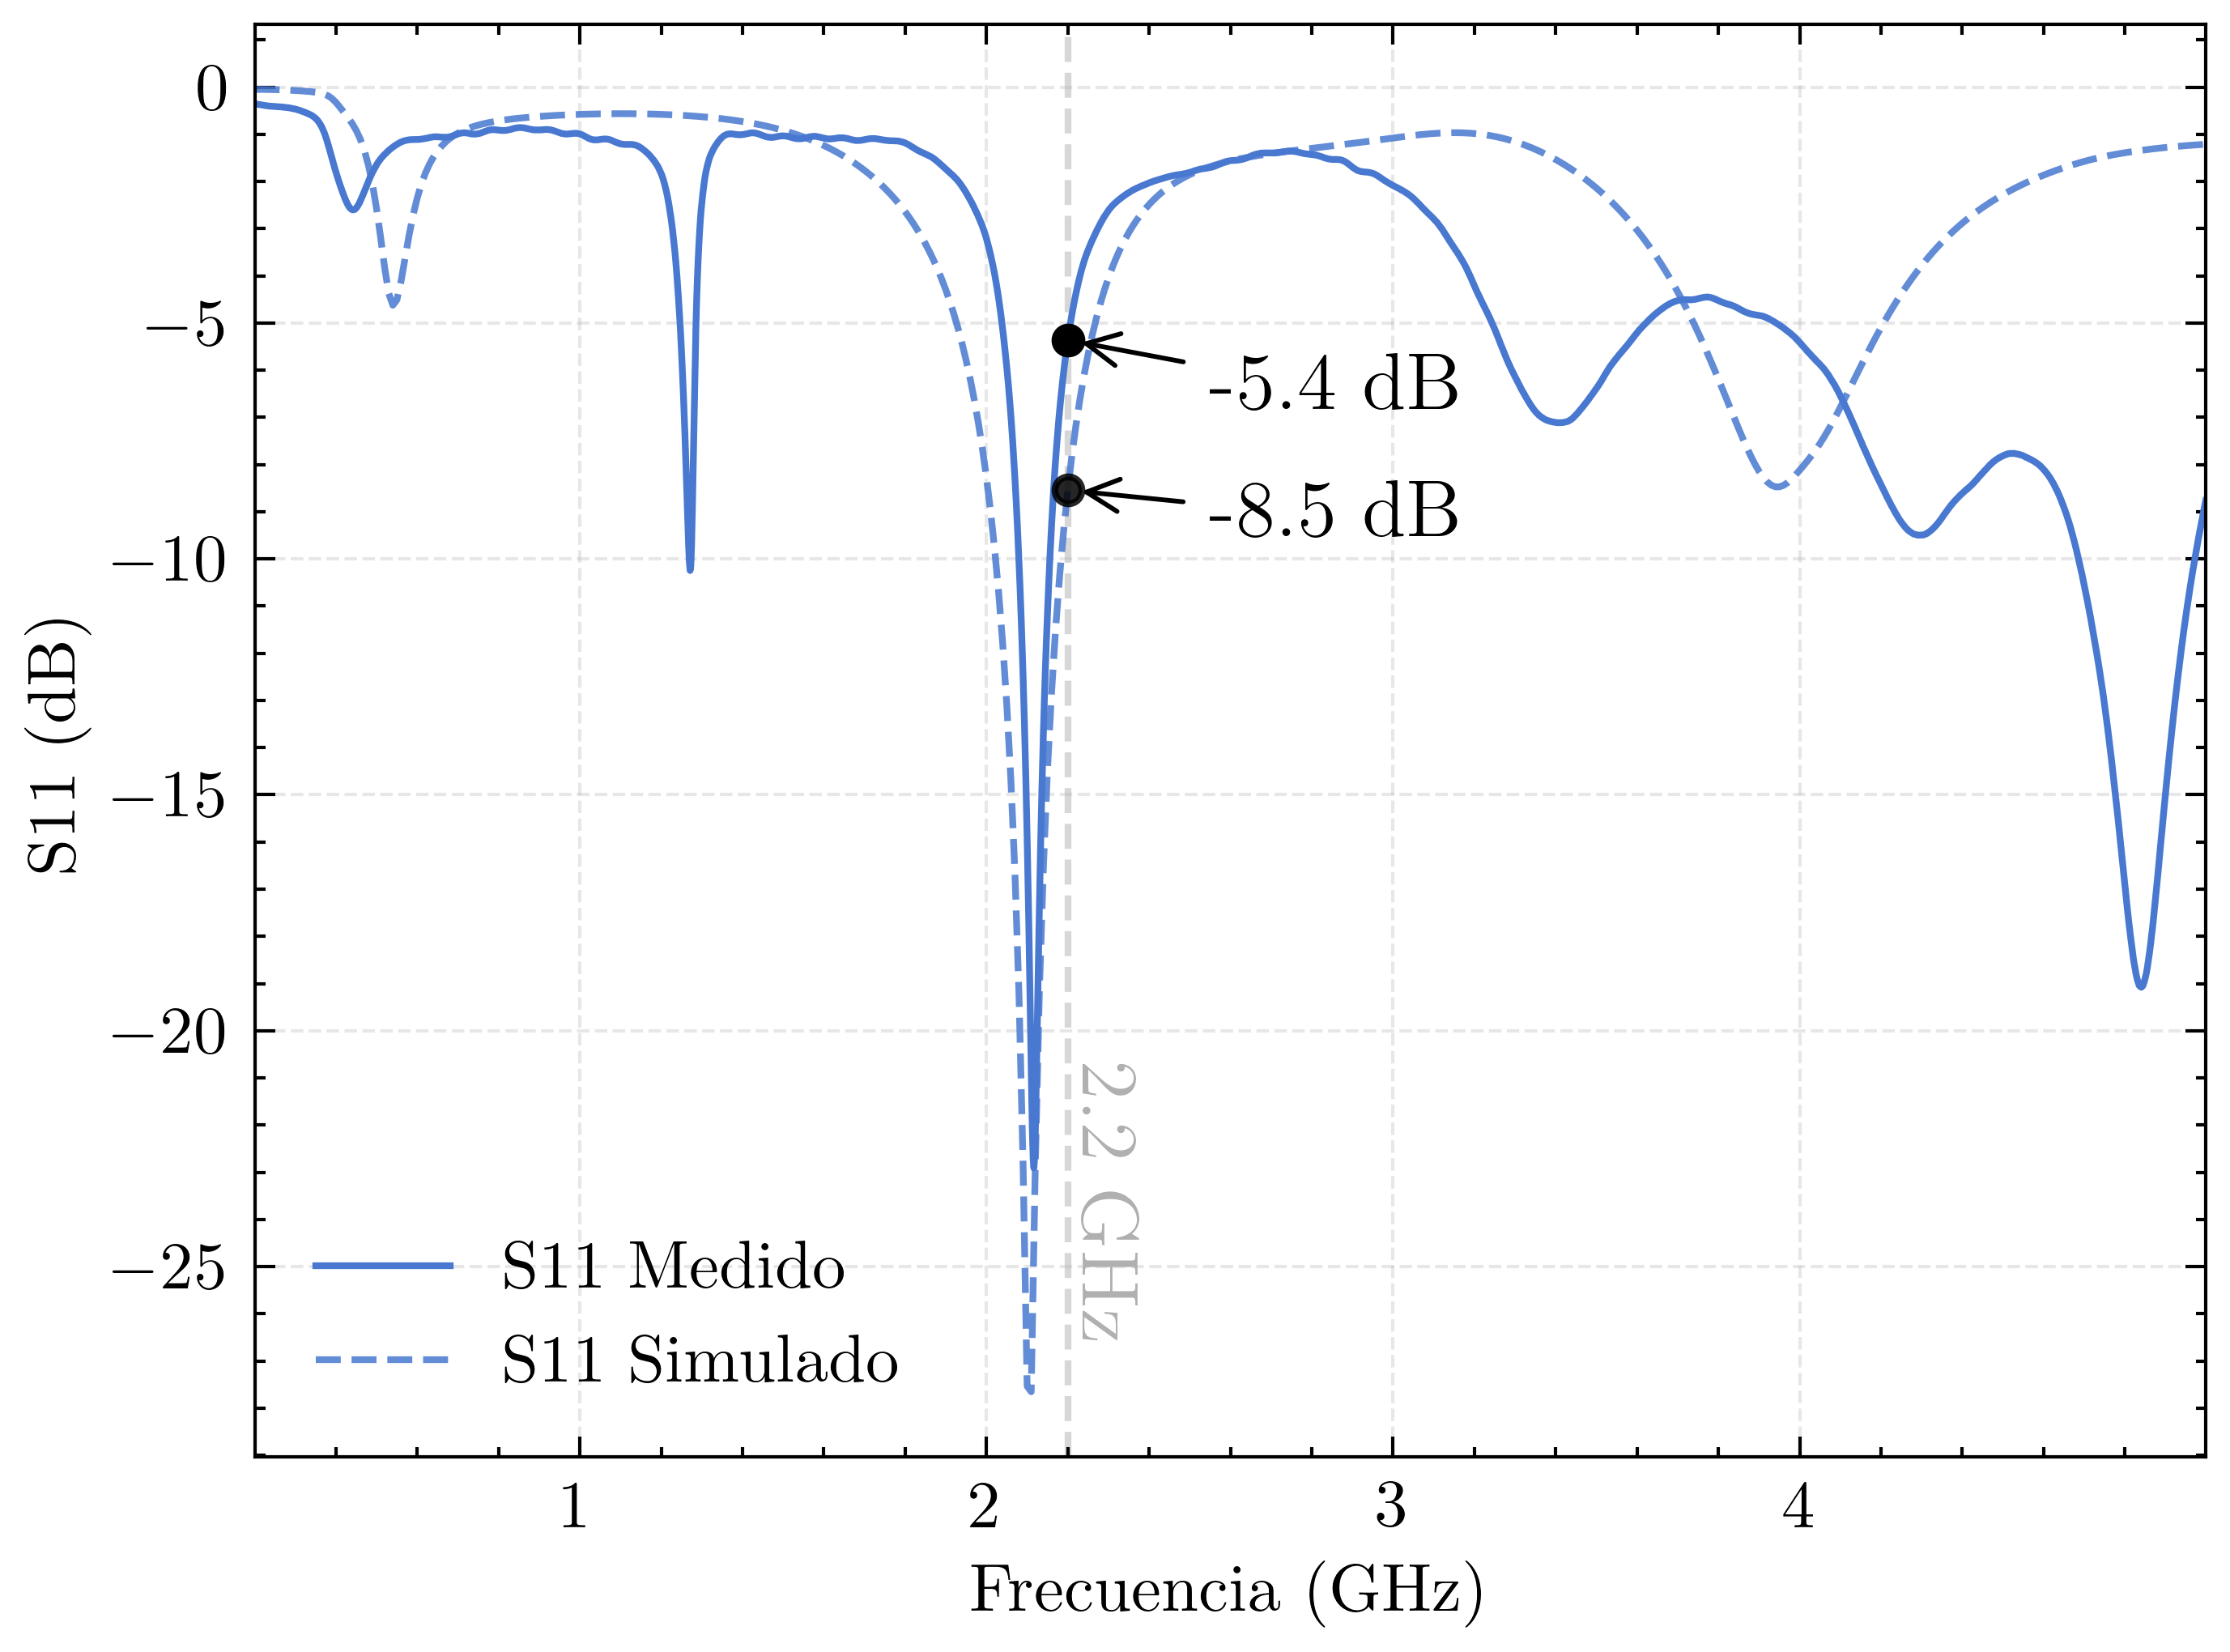
\includegraphics[width=0.7\linewidth]{imgs/s11_plot.png}
    \caption{Comparación entre el $S_{11}$ simulado (línea punteada) y medido (línea sólida) del amplificador de potencia fabricado.}
    \label{fig:s11_meas}
\end{figure}

\begin{figure}[H]
    \centering
    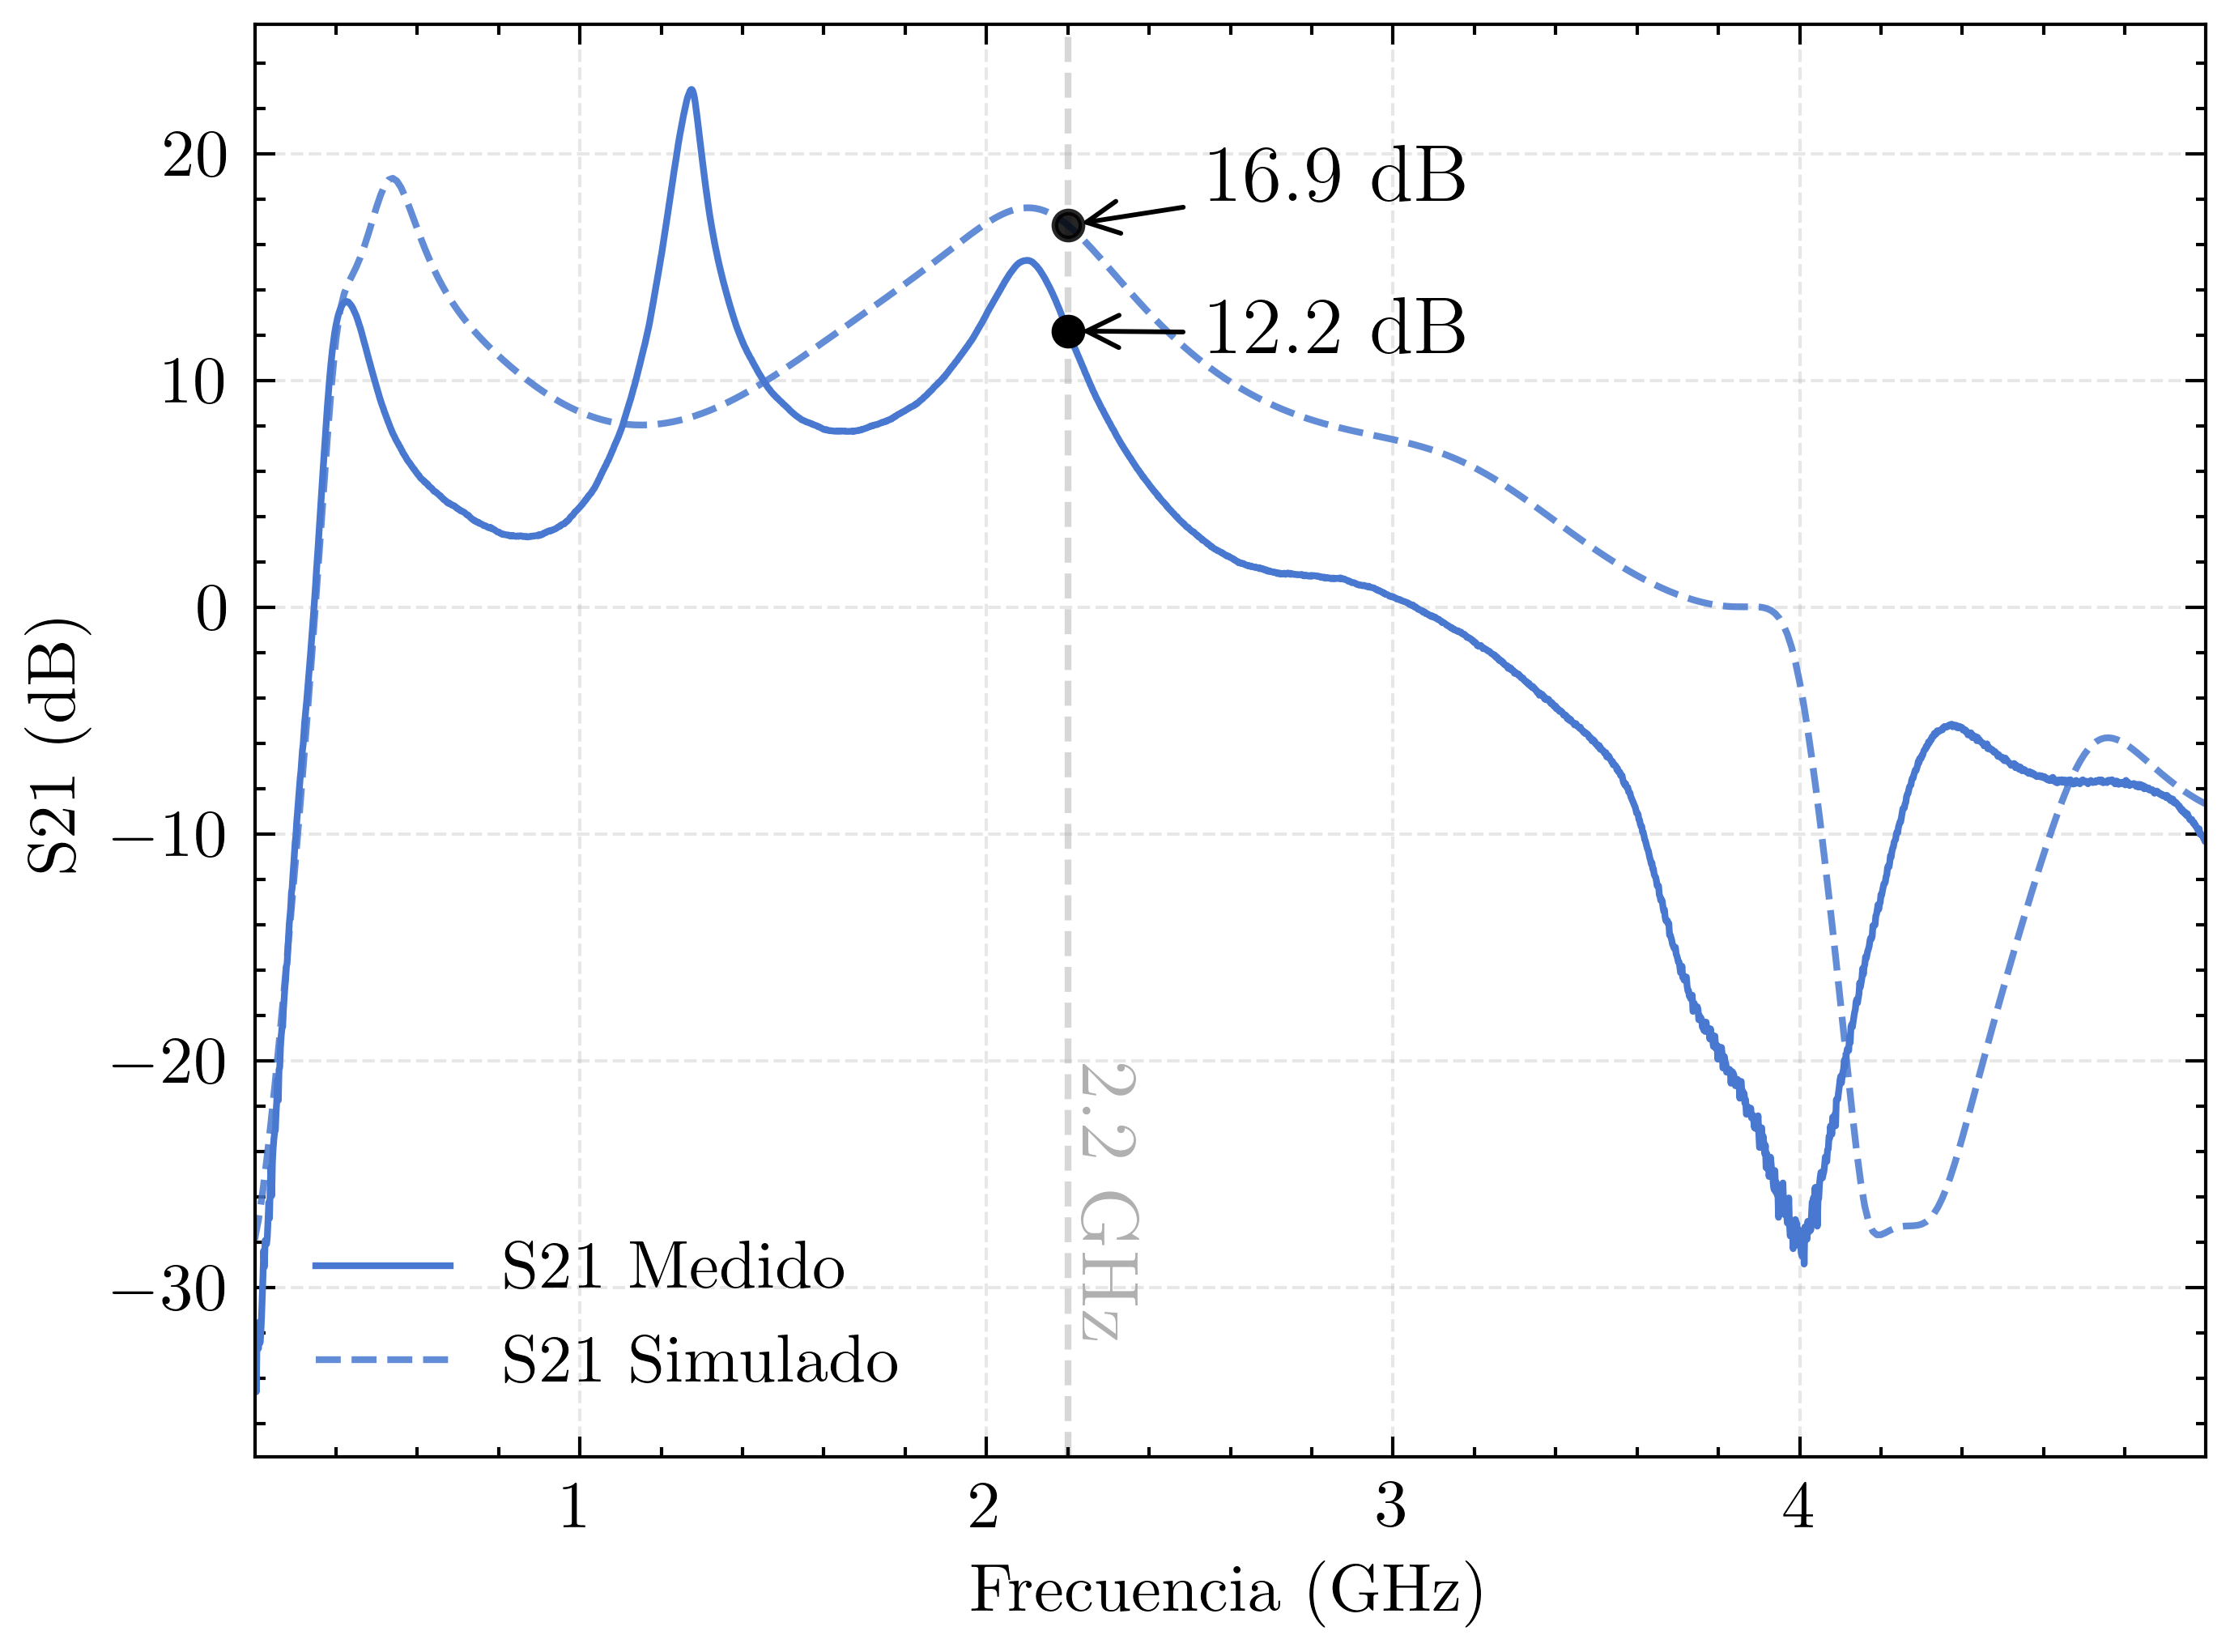
\includegraphics[width=0.7\linewidth]{imgs/s21_plot.png}
    \caption{Comparación entre el $S_{21}$ simulado (línea punteada) y medido (línea sólida) del amplificador de potencia fabricado.}
    \label{fig:s21_meas}
\end{figure}

La frecuencia central medida es de 2{,}11\,GHz, lo que corresponde a un desplazamiento de 90\,MHz respecto del objetivo de diseño de 2{,}2\,GHz. Este desplazamiento se atribuye a la inductancia equivalente serie (ESL) de las resistencias de la red de estabilidad, no contemplada en el modelo original. Al incorporar una ESL de 0{,}5\,nH por resistencia, valor consistente con datos publicados para resistencias de película fina en encapsulado 0603~\cite{VishayTN}, la frecuencia central simulada queda en concordancia con la medición. El comportamiento general de pequeña señal resulta consistente con la intención de diseño.

% -----------------------------------------------------------------------------------------------%
\subsection{Extracción del P1dB}
El punto de compresión de ganancia de 1\,dB (P1dB) constituye una figura de mérito clave para amplificadores de potencia, definido como el nivel de potencia de entrada en el cual la potencia de salida se desvía 1\,dB respecto de la respuesta lineal de pequeña señal extrapolada. Este punto delimita el límite de la región de operación lineal del amplificador~\cite{Pozar2012}.

La Figura~\ref{fig:p1db} muestra la potencia de salida medida en función de la potencia de entrada para la cadena completa de medición, compuesta por el amplificador driver y el amplificador bajo prueba. Dado que el amplificador driver ingresa en compresión dentro del rango de medición, el P1dB del dispositivo bajo prueba no puede leerse directamente de la curva de potencia de salida medida. Por este motivo, se aplicó la expresión de compresión en cascada de la ecuación~\eqref{eq:p1db_cascada}, presentada en la sección de metodología, que refiere la compresión de cada etapa a la entrada del sistema y combina sus contribuciones ponderadas inversamente por la ganancia de las etapas precedentes. El P1dB del amplificador bajo prueba se extrajo resolviendo esta expresión a partir de la ganancia y los valores de compresión conocidos de la etapa driver, obteniéndose un P1dB de 30{,}3\,dBm a una frecuencia de operación de 2{,}2\,GHz.

\begin{figure}[H]
    \centering
    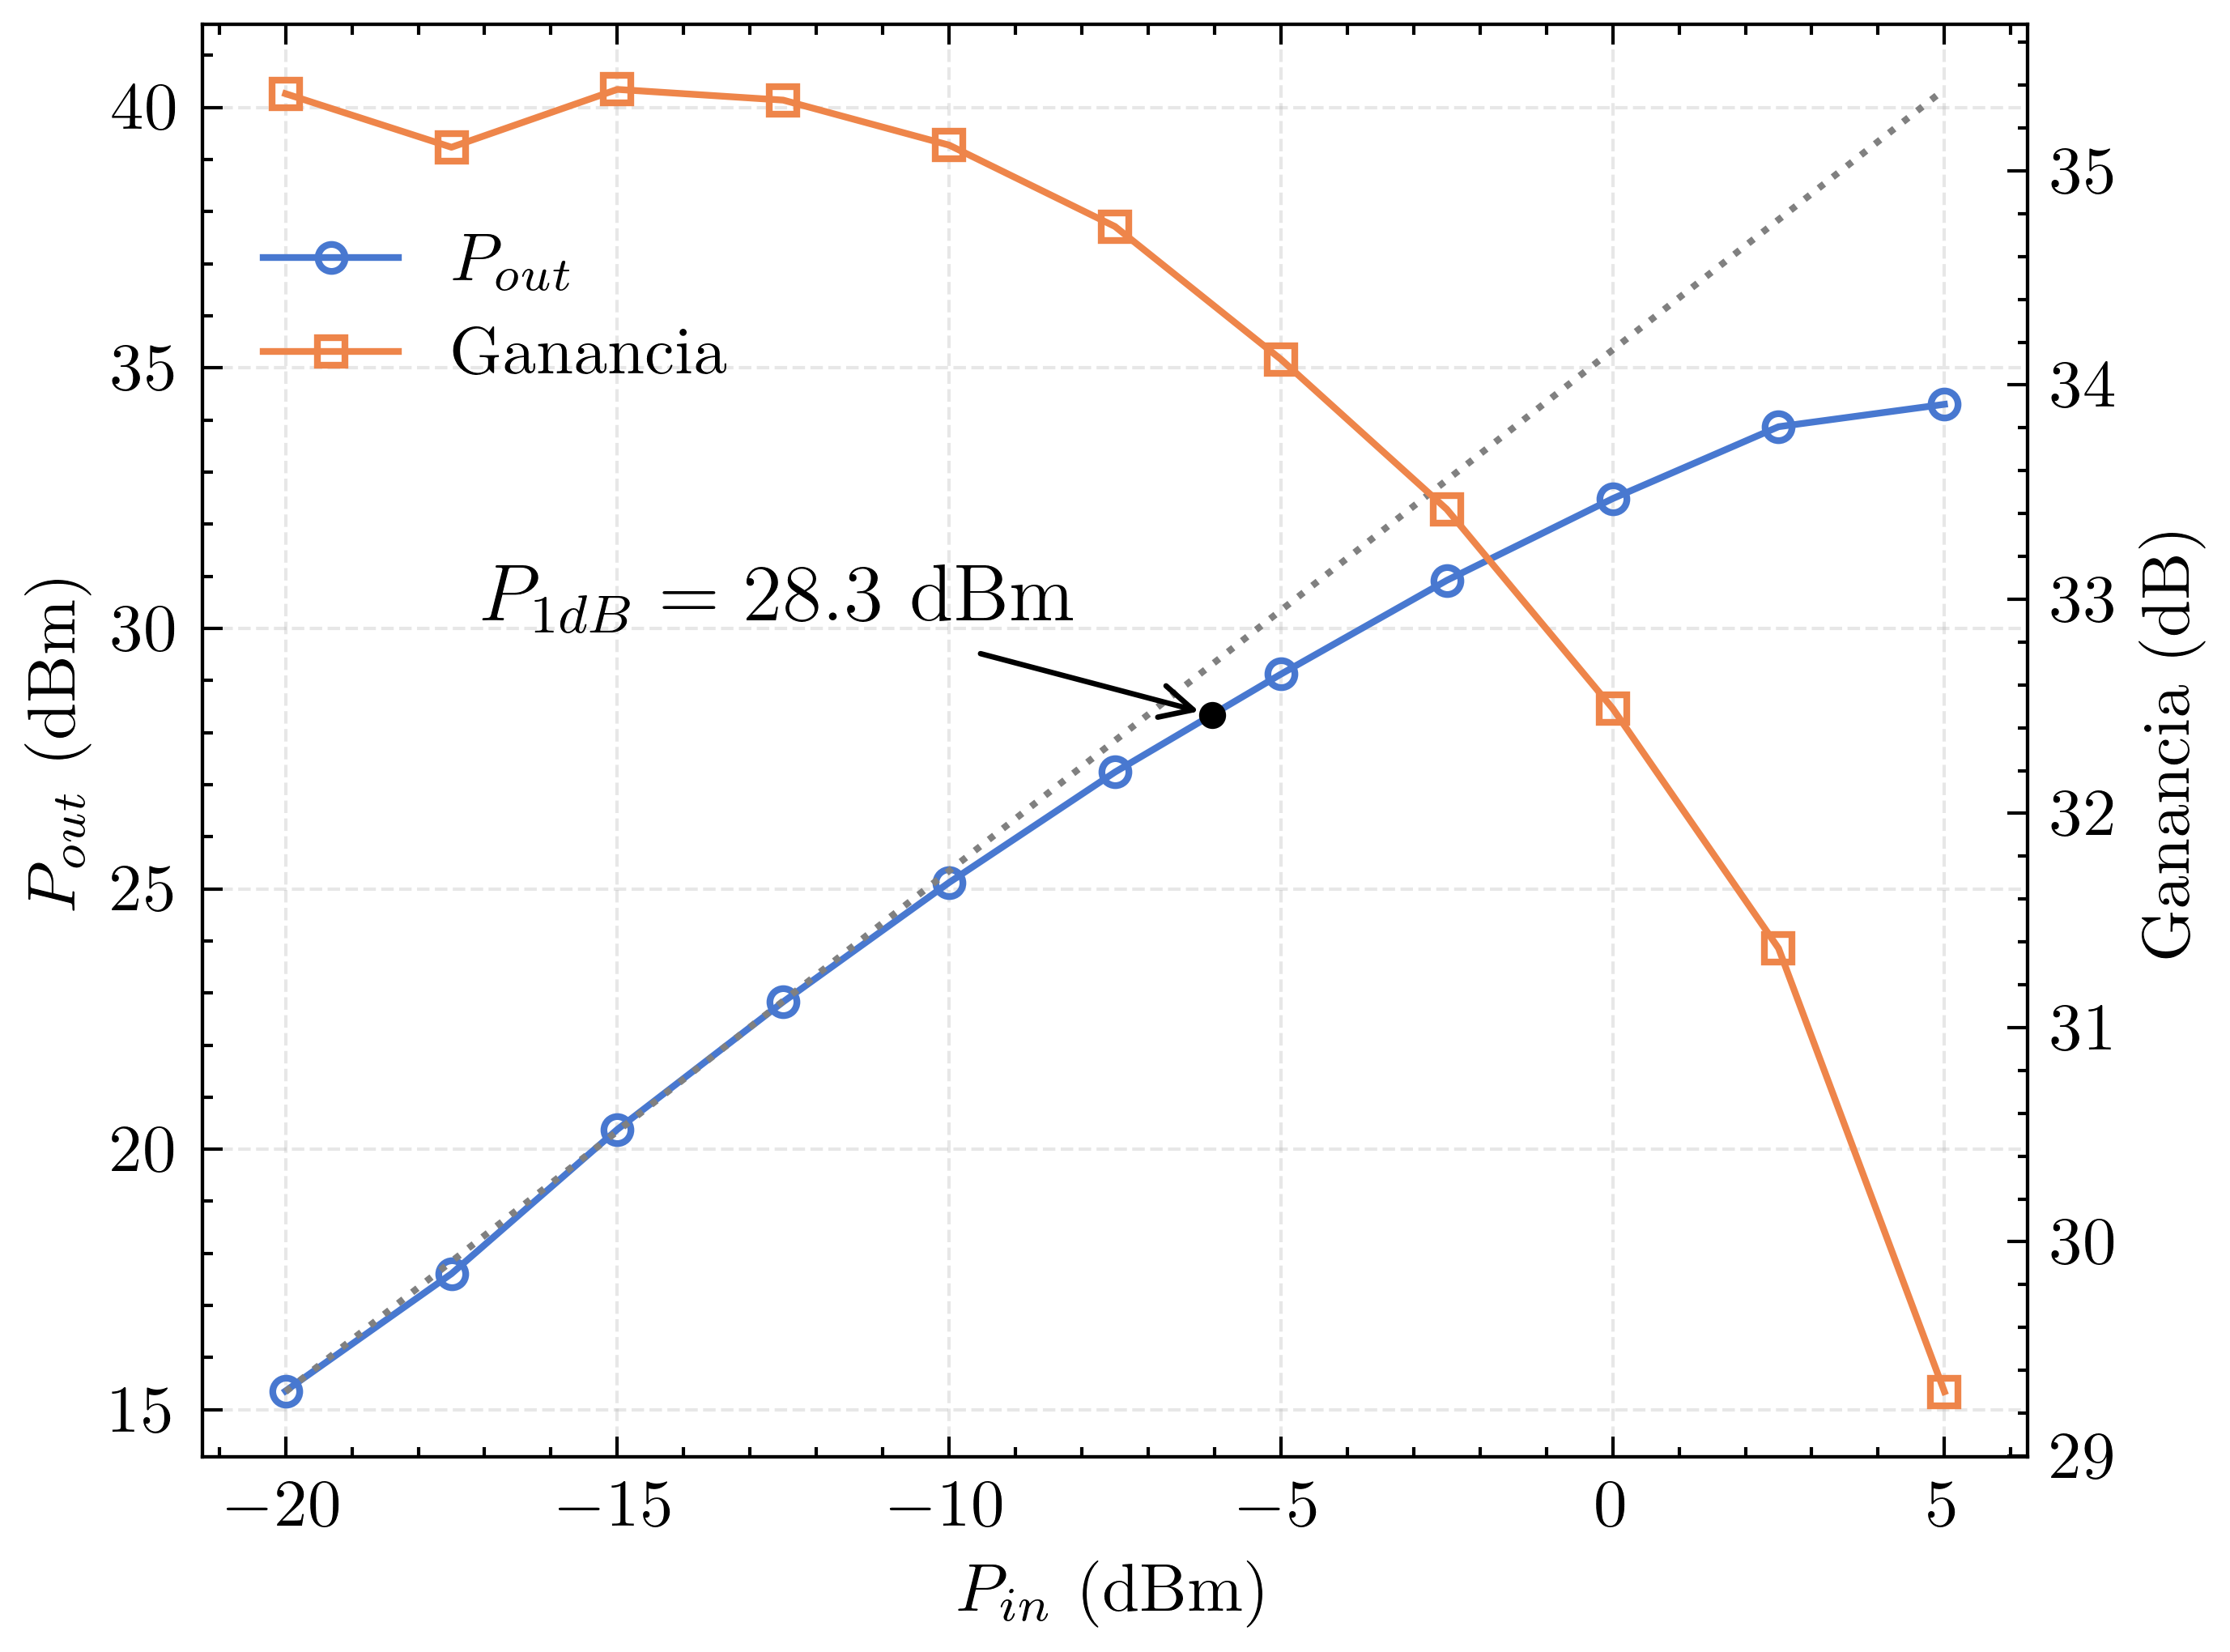
\includegraphics[width=0.8\linewidth]{imgs/p1db_plot.png}
    \caption{Potencia de salida medida (azul) y ganancia (naranja) en función de la potencia de entrada para la cadena driver-DUT. La línea punteada gris representa la característica de transferencia lineal ideal obtenida de la extrapolación de ganancia de pequeña señal.}
    \label{fig:p1db}
\end{figure}

% -----------------------------------------------------------------------------------------------%
\subsection{Ganancia, Eficiencia de Drain y Ancho de Banda}

% -----------------------------------------------------------------------------------------------%
\subsubsection{Ganancia}

La ganancia de pequeña señal del amplificador se extrajo a partir de la cadena de medición de potencia. La potencia de entrada y de salida en los terminales del amplificador se calcularon como

\begin{equation}
P_{in,PA} = P_{in,sys} + G_{driver}
\label{eq:pin_pa}
\end{equation}

\begin{equation}
P_{out,PA} = P_{out,sys} + |A_{att}|
\label{eq:pout_pa}
\end{equation}

donde $P_{in,sys}$ es la potencia de entrada del sistema, $G_{driver}$ es la ganancia de la etapa driver, $P_{out,sys}$ es la potencia de salida medida del sistema y $|A_{att}|$ es la atenuación total de la cadena de atenuadores, con todas las magnitudes expresadas en dBm y dB respectivamente. La ganancia se calculó entonces como

\begin{equation}
G = P_{out,PA} - P_{in,PA}
\label{eq:gain_calc}
\end{equation}

Se obtuvo una ganancia de pequeña señal de 13{,}26\,dB.

% -----------------------------------------------------------------------------------------------%
\subsubsection{Eficiencia de Drain}
La eficiencia de drain ($\eta_D$) se evaluó en el punto de medición más cercano al punto de compresión de 1\,dB, correspondiente a una potencia de salida de 30{,}92\,dBm, y se calculó como

\begin{equation}
\eta_D = \frac{P_{out,PA}}{P_{DC}} \times 100\%
\label{eq:drain_eff}
\end{equation}

donde $P_{out,PA}$ es la potencia de salida entregada por el amplificador y $P_{DC}$ es la potencia de continua consumida. Se obtuvo una eficiencia de drain de 32{,}94\%.

% -----------------------------------------------------------------------------------------------%
\subsubsection{Ancho de Banda}
El ancho de banda de operación se determinó a partir de la respuesta medida de $S_{11}$. Se identificaron los dos puntos de frecuencia en los cuales $S_{11}$ cruza el umbral de $-10$\,dB dentro de la región de interés, y el ancho de banda se definió como la diferencia entre ambos, obteniéndose un valor de 70\,MHz.

% -----------------------------------------------------------------------------------------------%
\subsection{Distorsión Armónica Medida}
El segundo y el tercer armónico se midieron con una potencia de entrada $P_{in} = 20\,\text{dBm}$, aproximadamente en el punto de operación correspondiente al P1dB, representando la condición no lineal de peor caso durante la operación normal del amplificador. El rechazo del segundo armónico fue de 26{,}74\,dBc y el rechazo del tercer armónico fue de 42{,}21\,dBc. Estos valores representan el desempeño mínimo esperado en operación lineal por debajo del P1dB. El contenido armónico medido difiere del modelo de simulación, lo cual se atribuye a un desplazamiento en frecuencia de la banda de rechazo del filtro de salida. Este efecto puede observarse en la respuesta de transmisión directa del amplificador ($S_{21}$), donde la banda de rechazo del filtro de salida aparece desplazada hacia frecuencias menores.

% -----------------------------------------------------------------------------------------------%
\subsection{OIP3 Medido}
El punto de intercepción de tercer orden a la salida (OIP3) es otro parámetro que caracteriza el comportamiento no lineal del amplificador. Constituye una figura de mérito que indica la potencia de salida en la cual los productos de intermodulación de tercer orden (IM3) resultan comparables con la señal fundamental. Su relevancia radica en que los IM3 se encuentran típicamente dentro de la banda de operación. El OIP3 es un punto teórico definido como la intersección entre la extrapolación de la curva de transferencia de potencia de salida respecto de la potencia de entrada, con pendiente unitaria en escala log-log, y la extrapolación de la respuesta de los IM3 en función de la potencia de entrada, cuya pendiente es de 3\,dB/dB en la misma escala~\cite{Pozar2012}.

El OIP3 se determinó para la cadena conjunta del driver y el amplificador de potencia. La Figura~\ref{fig:oip3} muestra el OIP3 de la cadena para un amplio rango de frecuencias. De manera análoga al caso del P1dB, la no linealidad del amplificador driver afecta el OIP3 de la cadena. Por este motivo, el valor de OIP3 correspondiente al dispositivo bajo prueba se obtuvo mediante la ecuación~\eqref{eq:oip3_cascada}

\begin{equation}
OIP3_{Sys} = \left( \frac{1}{OIP3_{N-1} \cdot G_N} + \frac{1}{OIP3_N} \right)^{-1} \text{[mW]}
\label{eq:oip3_cascada}
\end{equation}

Se obtuvo un OIP3 de 39,83\,dBm. Este valor resulta consistente con la relación experimental esperada entre el P1dB y el OIP3, donde el OIP3 suele ser de 10 a 15\,dB mayor que el P1dB~\cite{Pozar2012}.

\begin{figure}[H]
    \centering
    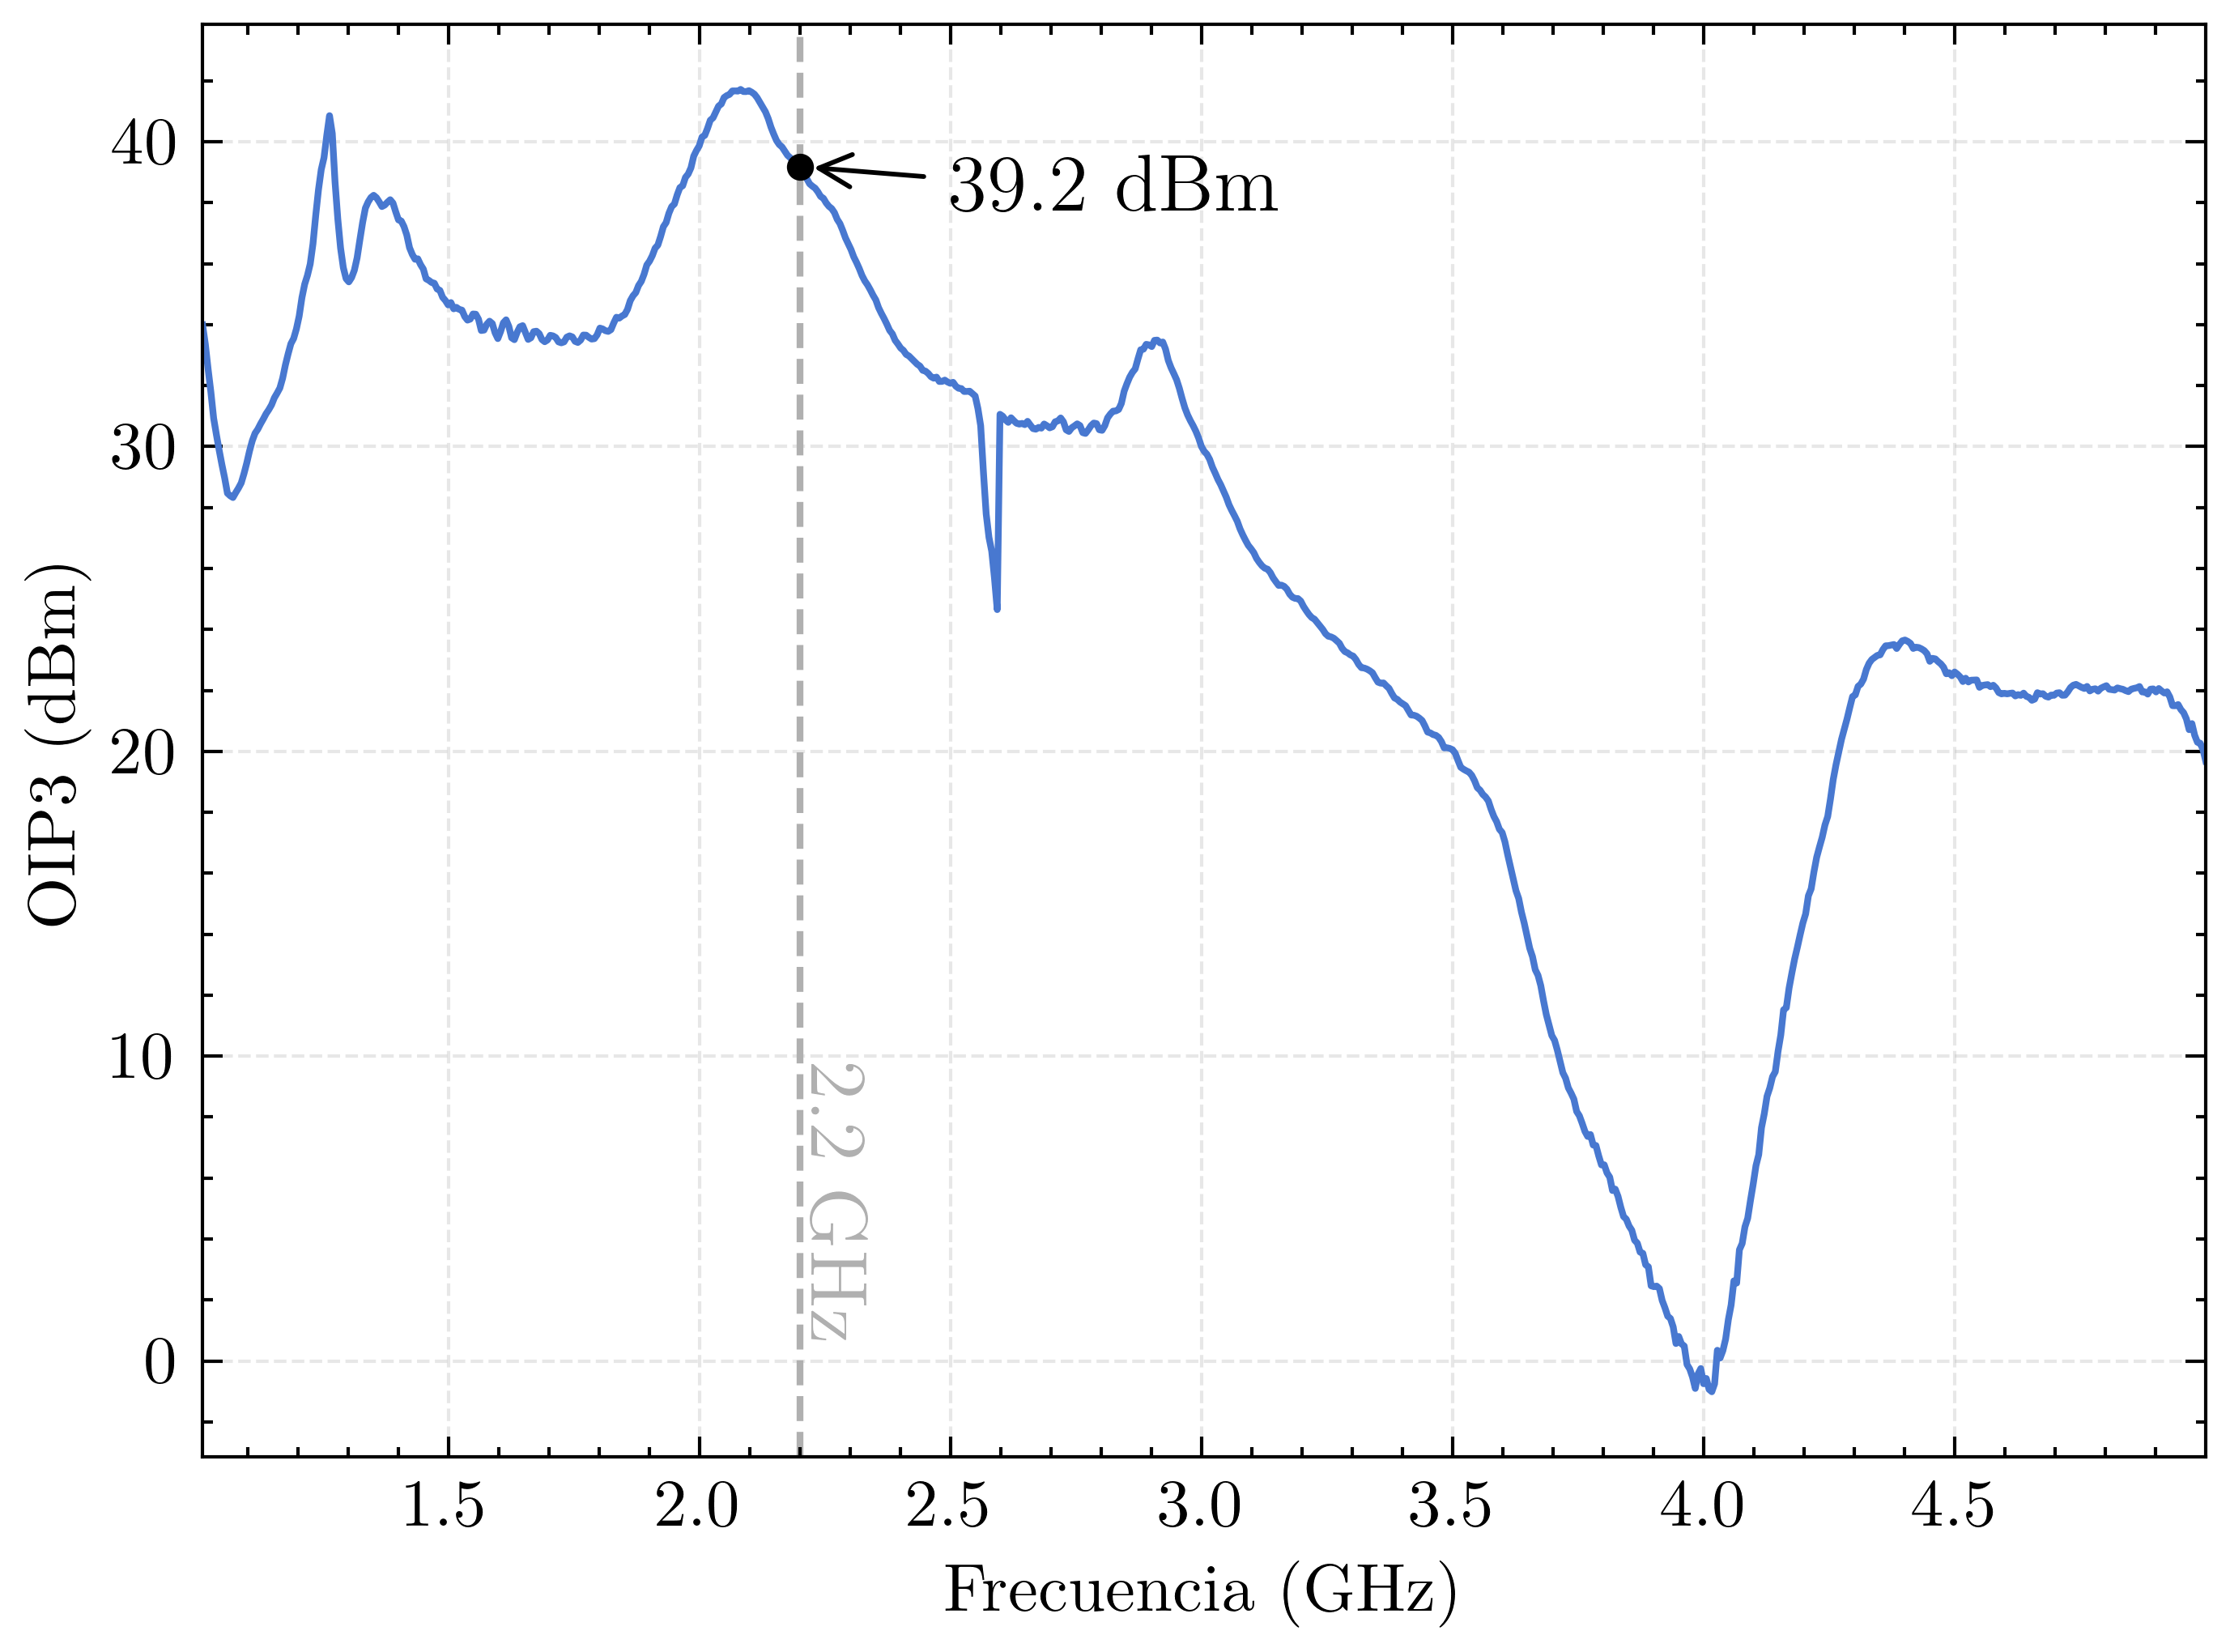
\includegraphics[width=0.8\linewidth]{imgs/oip3_plot.png}
    \caption{Barrido en frecuencia del punto de intercepción de tercer orden a la salida (OIP3) medido para la cadena driver-DUT.}
    \label{fig:oip3}
\end{figure}

% -----------------------------------------------------------------------------------------------%
\subsection{Resumen de Resultados}
La Tabla~\ref{tab:resumen_resultados} resume los parámetros de desempeño clave medidos del amplificador fabricado, presentando una vista consolidada de los resultados de caracterización descritos a lo largo de esta sección.

\begin{table}[H]
    \centering
    \caption{Resumen de Desempeño Medido del Amplificador de Potencia RF}
    \label{tab:resumen_resultados}
    \begin{tabular}{|l|c|}
        \hline
        \textbf{Parámetro} & \textbf{Valor} \\
        \hline
        Frecuencia Central & 2,11\,GHz \\
        \hline
        Ancho de Banda (BW) & 70\,MHz \\
        \hline
        Punto de Compresión de 1\,dB (P1dB) & 30,30\,dBm \\
        \hline
        Intercepción de Tercer Orden (OIP3) & 39,83\,dBm \\
        \hline
        Ganancia de Pequeña Señal & 13,26\,dB \\
        \hline
        Eficiencia de Drain & 32,94\% @ $P_{out} = 30{,}92\,$ dBm \\
        \hline
        VSWR & $<1{,}92$:1 \\
        \hline
    \end{tabular}
\end{table}